% Relative path to the directory with common files for documentation.
\newcommand{\commondocpath}{../../../common/doc}

\documentclass[a4paper,english,11pt,oneside]{article}
\usepackage{amssymb}
\usepackage[T1]{fontenc}
\usepackage{libertine}  
\renewcommand*\familydefault{\sfdefault}
\usepackage{tabularx}
\usepackage{amsmath}
\usepackage{adjustbox}
\usepackage{multicol}
\usepackage{mathtools}
\usepackage[utf8]{inputenc}
\usepackage{microtype}
\usepackage{geometry}
\geometry{textheight=235mm,textwidth=180mm,headsep=12mm,tmargin=20mm}
\usepackage{babel}
\usepackage{eurosym}
\usepackage{blindtext}
\usepackage{graphicx}
\usepackage{textpos}                         % placing boxes at absolute positions
\usepackage{xcolor} 
\usepackage{gensymb}
\widowpenalty 10000
\clubpenalty 10000
\usepackage{makeidx}
\usepackage{caption}

\definecolor{light-gray}{gray}{0.95}
\definecolor{dark-green}{HTML}{3C8031}

\usepackage{listings}
\lstset{
	backgroundcolor=\color{light-gray},
	basewidth=0.55em,
	basicstyle=\footnotesize\ttfamily,        % the size of the fonts that are used for the code
	breaklines=true,
	commentstyle=\color{dark-green}, % comment color
	frame=none,
	keywordstyle=\color{blue}, % keyword color
	language=C++,
	numbers=left, % display line numbers on the left
	tabsize=4, % tab space width
	showstringspaces=false, % don't mark spaces in strings
	stringstyle=\color{red} % string color
} 
\usepackage{float}   
\usepackage{lastpage}

\usepackage[onehalfspacing]{setspace}
\usepackage{multirow}
\usepackage{bigstrut}

\usepackage{array,booktabs}
\usepackage{color} 

\usepackage{colortbl}
\usepackage[pdfborder={0 0 0}]{hyperref}
\usepackage{url}


\usepackage{makecell}
\definecolor{ibeo_red}{cmyk}{0.13,0.99,0.87,0.03}
\definecolor{ibeo_grey}{cmyk}{0.35,0.28,0.26,0}
\definecolor{ibe_antrazit}{cmyk}{0.72,0.65,0.59,0.50}

\usepackage{chngcntr}
\counterwithin{figure}{section}
\counterwithin{table}{section}

\setlength{\parindent}{0pt}

%---------------------------------------------------------------------------------------------------
% Header Ibeo % Footer
%---------------------------------------------------------------------------------------------------
\def\title#1{\gdef\@title{#1}\gdef\THETITLE{#1}}
\pagenumbering{arabic} 
\usepackage{fancyhdr}
\addtolength{\headheight}{2cm} % make more space for the header
\pagestyle{fancyplain} % use fancy for all pages except chapter start
\fancyheadoffset{1.5cm}
\lhead{\hspace{1.5cm} 
\includegraphics[height=1.6cm]{\commondocpath/images/ibeo_logo.jpg}} % left logo
\chead{}
\rhead{Page \thepage\ of \pageref{LastPage} \hspace*{1.5cm}}
\fancyfootoffset{1.5cm}
\lfoot{\hspace{1.5cm}  \THETITLE}
\cfoot{}
\rfoot{
\includegraphics[width=7cm]{\commondocpath/images/ibeo_slogan.png}\hspace*{1.5cm}}
\renewcommand{\headrule}{\hbox to\headwidth{%
  \color{ibeo_red}\leaders\hrule height \headrulewidth\hfill}}
\renewcommand{\footrule}{\hbox to\headwidth{%
  \color{ibeo_red}\leaders\hrule height \headrulewidth\hfill}}
\renewcommand{\headrulewidth}{2pt}
\renewcommand{\footrulewidth}{2pt} 

\newcommand{\bild}[3]{
  \begin{figure}[!hbt]
    \centering
      \vspace{1ex}
	 \fbox{
      \includegraphics[width=#2]{images/#1}}
      \caption{#3}
      \label{fig:#3}
    \vspace{1ex}
  \end{figure}
}
\newcommand{\bildref}[4]{
  \begin{figure}[!hbt]
    \centering
      \vspace{1ex}
	\frame{
      \includegraphics[width=#2]{images/#1}}
      \caption{#3}
      \label{fig:#4}
    \vspace{1ex}
  \end{figure}
}



\newcommand{\symDANGER}[1]{
\begin{center}
	\begin{minipage}[c]{0.1\textwidth}
		\vspace{0pt}
		
\includegraphics[width=\textwidth]{\commondocpath/images/danger.png}
	\end{minipage}
	\begin{minipage}[c]{0.8\textwidth}
	\vspace{0pt}
	\begin{tabular}{| >{\centering\arraybackslash}m{13cm} |}
		\hline
		\cellcolor{red} \color{white} \begin{bfseries}DANGER\end{bfseries} \normalfont  \\
		\cline{1-1}
		{#1} \\
		\hline
	\end{tabular}
	\end{minipage}
\end{center}
}

\newcommand{\symWARNING}[1]{
\begin{center}
	\begin{minipage}[c]{0.1\textwidth}
		\vspace{0pt}
		
\includegraphics[width=\textwidth]{\commondocpath/images/danger.png}
	\end{minipage}
	\begin{minipage}[c]{0.8\textwidth}
	\vspace{0pt}
	\begin{tabular}{| >{\centering\arraybackslash}m{13cm} |}
		\hline
		\cellcolor{orange} \color{black} \begin{bfseries}WARNING\end{bfseries} \normalfont  \\
		\cline{1-1}
		{#1} \\
		\hline
	\end{tabular}
	\end{minipage}
\end{center}
}

\newcommand{\symCAUTION}[1]{
\begin{center}
	\begin{minipage}[c]{0.1\textwidth}
		\vspace{0pt}
		
\includegraphics[width=\textwidth]{\commondocpath/images/danger.png}
	\end{minipage}
	\begin{minipage}[c]{0.8\textwidth}
	\vspace{0pt}
	\begin{tabular}{| >{\centering\arraybackslash}m{13cm} |}
		\hline
		\cellcolor{yellow} \color{black} \begin{bfseries}CAUTION\end{bfseries} \normalfont  \\
		\cline{1-1}
		{#1} \\
		\hline
	\end{tabular}
	\end{minipage}
\end{center}
}

\newcommand{\symCAUTIONHAND}[1]{
\begin{center}
	\begin{minipage}[c]{0.1\textwidth}
		\vspace{0pt}
		
\includegraphics[width=\textwidth]{\commondocpath/images/caution.png}
	\end{minipage}
	\begin{minipage}[c]{0.8\textwidth}
	\vspace{0pt}
	\begin{tabular}{| >{\centering\arraybackslash}m{13cm} |}
		\hline
		 \cellcolor{yellow} \color{black} \vspace{1mm}\begin{bfseries}CAUTION\end{bfseries} \normalfont   \\
		\cline{1-1}
		#1 \\
		\hline
	\end{tabular}
	\end{minipage}
\end{center}
}

\newcommand{\symNOTE}[1]{
\begin{center}
	\begin{minipage}[c]{0.1\textwidth}
		\vspace*{0pt}
		\hspace*{0.4cm}
\includegraphics[width=0.3\textwidth]{\commondocpath/images/note.png}
	\end{minipage}
	\begin{minipage}[c]{0.8\textwidth}
	\vspace*{0pt}
	\begin{tabular}{| >{\centering\arraybackslash}m{13cm} |}
		\hline
		\cellcolor{blue} \color{white} \vspace{1mm}\begin{bfseries}NOTE\end{bfseries} \normalfont    \\
		\cline{1-1}
		\textit {#1} \\
		\hline
	\end{tabular}
	\end{minipage}
\end{center}
}

\newcommand{\IbeoTabelle}{
	\begin{table}[!htbp]
	\begin{center}
	\renewcommand{\arraystretch}{1.5}
		\begin{tabular}{| m{4cm} | m{3cm} | m{2cm} | m{6.6cm} |}
		\hline
		\cellcolor{ibeo_red} \textcolor{white}{\textbf{Parameter}} & \cellcolor{ibeo_red} \textcolor{white}{\textbf{Data type}} & \cellcolor{ibeo_red} \textcolor{white}{\textbf{Default}} & \cellcolor{ibeo_red} \textcolor{white}{\textbf{Description}} \\
		\hline
		ObjectListDataType & Hex16 & 0x2280 & Chose 0x2225 for backward compability, refer to the Customer Ethernet Document for contents and structure of the datatypes \\
		\hline
		VehicleStateDataType & Hex16 & 0x2807 & Chose 0x 2806 for backward compability, refer to the Customer Ethernet Document for contents and structure of the datatypes\\
		\hline
	\end{tabular}
	\caption{DataTypeSelectorWorker Configuration}
	\label{table:DataTypeSelectorWorker Configuration}
	\end{center}
	\end{table}
}
\urlstyle{same}


\usepackage{scrextend}

\usepackage{xcolor}

\usepackage[most]{tcolorbox}
\tcbset{
	frame code={}
	center title,
	left=0pt,
	right=0pt,
	top=0pt,
	bottom=0pt,
	colback=light-gray,
	colframe=white,
	width=\dimexpr\textwidth\relax,
	enlarge left by=0mm,
	boxsep=5pt,
	arc=0pt,outer arc=0pt,
}

\usepackage{fancyvrb}
\fvset{tabsize=4}

\usepackage{longtable}

\newcommand{\sourcecode}[1]{\begin{footnotesize}\colorbox{light-gray}{\texttt{\detokenize{#1}}}\end{footnotesize}}
\newcommand{\fullref}[1]{\ref{#1}-\nameref{#1}}

\begin{document}
\title{Introduction to Logging Services in the ibeoSDK}
\newpage

\newpage
\fancypagestyle{plain}{%
\lhead{} 
\chead{}
\rhead{}
\lfoot{}
\cfoot{}
\rfoot{}

\renewcommand{\headrulewidth}{0.0pt} 
\renewcommand{\footrulewidth}{0.0pt} }
\thispagestyle{plain}

\begin{center}
\vspace*{3cm}

\includegraphics[height=3cm]{\commondocpath/images/ibeo_logo.jpg}
\vspace*{\fill}
\end{center}

\newpage

\fancypagestyle{plain}{%
\fancyheadoffset{1.5cm}
\lhead{\hspace{1.5cm} 
\includegraphics[height=1.6cm]{\commondocpath/images/ibeo_logo.jpg}} % left logo
\chead{}
\rhead{}
\lfoot{}
\cfoot{}
\rfoot{
\includegraphics[width=7cm]{\commondocpath/images/ibeo_slogan.png} \hspace{1.5cm}}
\renewcommand{\headrule}{\hbox to\headwidth{%
  \color{ibeo_red}\leaders\hrule height \headrulewidth\hfill}}
\renewcommand{\footrule}{\hbox to\headwidth{%
  \color{ibeo_red}\leaders\hrule height \headrulewidth\hfill}}
\renewcommand{\headrulewidth}{2pt}
\renewcommand{\footrulewidth}{2pt} }


\thispagestyle{plain}
\vspace*{6cm}
\begin{bfseries}
\begin{huge}
\huge \bfseries \noindent Ibeo SDK - Logging Services\\ [1.5cm]
\huge \bfseries User Manual
\end{huge}
\end{bfseries}
\newpage
\thispagestyle{plain}

\newpage
\begin{bfseries} 
\null
\vfill
\begin{centering}Ibeo Automotive Systems GmbH\\
Merkurring 60-62\\
D - 22143 Hamburg\\
Phone: +49 - (0) 40 298 676 - 0\\
Fax: +49 - (0) 40 298 676 - 10\\
E-mail: \href{mailto:info@ibeo-as.com}{info@ibeo-as.com}
\vspace*{1.0cm}
 
Copyright\\
\mdseries 
All information contained in this documentation has been collected with utmost care and been checked for conformance with the ibeo LUX and programs. Nevertheless, minor variations cannot be excluded entirely. Necessary corrections will be documented in subsequent versions. The manufacturer reserves the right to this User Manual. Therefore, reproduction, copying, distribution or use for competitive purposes of this User Manual, as a whole or partially, is forbidden unless the manufacturer has given written consent.
Printing this user manual for personal use is permitted.
copyright© 2016
\end{centering}
\end{bfseries}

\newpage
\thispagestyle{plain}
\section*{Version History}
\begin{table}[H]
\centering
	\begin{tabular}{| p{3cm} | p{2cm} | p{10cm} |}
	\multicolumn{1}{c}{\textbf{Date}} & \multicolumn{1}{c}{\textbf{Version}} & \multicolumn{1}{c}{\textbf{Changes}}\\
	\hline
	20-Feb-2019 & 1.0 & Initial Version of this manual \\
	\hline
	\end{tabular}
	\caption{Version History}
	\label{tab:version history}
\end{table}
\clearpage


\thispagestyle{plain}
\tableofcontents


\newpage

%===================================================
\section{Introduction}
%===================================================

The ibeoSDK Logging Services are used to output log statements that aid debugging the code. It may be the only way of getting information about the status of the application e.g. when it is not possible to use a debugger. These services are not only used inside the SDK itself but are open to applications too. Please refer to section \fullref{sec:api} for how to use the Logging Services API.\\
\\
The following picture shows the general architecture of the Ibeo SDK Logging Services:

\begin{figure}[h]
	\centering
	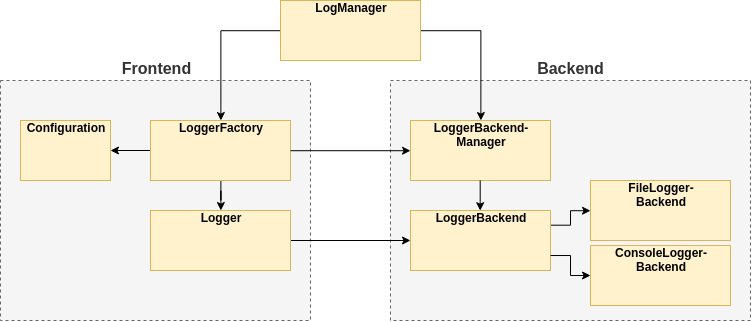
\includegraphics[scale=0.5]{images/logging_architecture.png}
	\caption{Architecture}
\end{figure}

An application uses Logger instances from the frontend to send messages of a given severity defined by the LogLevel to the logging system. To create a logger, the application chooses a unique identifier which is formatted like a C++ class name with namespace: e.g. \sourcecode{ibeo::common::logging::Logger} and calls the \sourcecode{createLogger} method from the \sourcecode{LogManager} class. The number of loggers an application can create is not limited by the Logging Services. So, it is possible to use a separate logger for each class or even for each class instance (e.g. if the class name is suffixed by an index or ID). The more loggers an application uses, the finer the logging can be controlled (see section \fullref{sec:configuration}).\\
A special logger is the global logger which can be retrieved using the \sourcecode{LogManager}'s \sourcecode{globalLogger} method. This instance can be used to quickly log messages without worrying about creating a logger. The downside is, that only one log level can be set for all messages sent through this logger.\\

The backend part of the logging system receives the log messages, filters them according to the currently set log level, and processes them. There are predefined logging backends for printing the log messages to the console (\sourcecode{ConsoleLoggerBackend}) or to file (\sourcecode{FileLoggerBackend}). Each backend is identified by a unique class ID. An application can create additional backends (e.g. for writing log messages into GUI window or a database). This is covered in section \fullref{sec:custombackends}.

\newpage



%===================================================
\section{API} \label{sec:api}
%===================================================

%---------------------------------------------------
\subsection{Prerequisites}
%---------------------------------------------------
The ibeoSDK Logging Services consist of quite a number of classes with their corresponding header files. For convenience, there is a single include file \path{ibeo/common/logging/logging.hpp} that contains all necessary includes and some macro definitions (see section \fullref{sec:sendinglogmessages}).\\
All classes are defined in the C++ namespace \sourcecode{ibeo::common::logging}. To use them, they should be referenced by their fully qualified name (e.g. \sourcecode{ibeo::common::logging::LogManager}), by adding a using-directive (e.g. \sourcecode{using namespace ibeo::common::logging}), or with a namespace-alias-definition\\ (e.g. \sourcecode{namespace logging=ibeo::common::logging}). In the latter case, the corresponding class must be referenced through that alias (e.g. \sourcecode{logging::LogManager}).


%---------------------------------------------------
\subsection{Obtaining a Logger} \label{sec:obtainingalogger}
%---------------------------------------------------
The first task for a developer when writing log messages is to get a logger from the Logging Services. This can be achieved in two different ways:
\begin{itemize}
\item by using the Log Manager instance for creating a logger with a unique ID
\begin{lstlisting}[numbers=none]
LogManager& logManager=LogManager::getInstance();
LoggerSPtr logger=logManager.createLogger("ibeo::common::app::Foo");
\end{lstlisting}
Although the logger ID can be any string, it is recommended to use the name of the class (together with its namespace) that creates the logger. This makes configuring the Logging Service easier (see section \fullref{sec:configuration}).

\item or by using the global logger 
\begin{lstlisting}[numbers=none]
LoggerSPtr logger = LogManager::globalLogger();
\end{lstlisting}
The global logger is a predefined instance in the Logging Services with the ID\\ \sourcecode{ibeo::common::logging::GlobalLogger}.
\end{itemize}
 

%---------------------------------------------------
\subsection{Log Levels}\label{sec:loglevel}
%---------------------------------------------------
The Logging Services define the following log levels which are used to define the severity of log messages.
\begin{itemize}
	\item \textit{Critical} messages should be used for very important issues where it is most likely that the application is not running correctly any longer.
	\item \textit{Error} is for severe messages where it is likely that the application does not work as expected any more.
	\item \textit{Warning} messages indicate errors that have been recovered. It is most likely that the application still runs as expected.
	\item \textit{Info} is for general purpose information, e.g. about the application's status.
	\item \textit{Trace} messages should be used to log communication with external systems (e.g. a network or a database connection).
	\item \textit{Debug} is for all other messages helping debugging the code.
\end{itemize}

The log levels are listed from most to less important. If - for instance - the level of a logger is set to \textit{Info} in the configuration all messages with levels \textit{Critical}, \textit{Error}, \textit{Warning}, and \textit{Info} are forwarded to the backend while messages with levels \textit{Trace} and \textit{Debug} are filtered out. Messages with level \textit{Critical} cannot be disabled.

%---------------------------------------------------
\subsection{Sending Log Messages} \label{sec:sendinglogmessages}
%---------------------------------------------------
Once a logger is obtained, it can be used to send log information by creating a \sourcecode{LogMessage} object and sending it to the backend with the logger's \sourcecode{log} function.
\begin{lstlisting}[numbers=none]
MessageSPtr msg = std::make_shared<ibeo::common::logging::Message>
                  (__LINE__, __FUNCTION__, __FILE__, "Log text.");
log(LogLevel::Info, msg);
\end{lstlisting}

The \sourcecode{Message} object carries information about the name, file path, and line number of the function where the message is created (represented by the predefined C++ macros in the example above).\\
The \sourcecode{LOGMSG\_TEXT} macro can be used to shorten the creation of log messages:
\begin{lstlisting}[numbers=none]
log(LogLevel::Info, LOGMSG_TEXT("Log text."));
\end{lstlisting}

The log message text can be extended by using the stream output operator “<<” and IO manipulators. In this case the \sourcecode{LOGMSG} macro should be used instead:
\begin{lstlisting}[numbers=none]
log(LogLevel::Info, LOGMSG << "Magic number: 0x" << std::hex << std::setw(4)
                           << magicNumber);
\end{lstlisting}

There are also convenience functions for each log level, e.g.:
\begin{lstlisting}[numbers=none]
logger->warning(LOGMSG << "Log text.");
\end{lstlisting}

As an alternative, the following macros can be used:
\begin{lstlisting}[numbers=none]
LOGCRITICAL(logger, LOGMSG << "Log text.");
LOGERROR(logger, LOGMSG << "Log text.");
LOGWARNING(logger, LOGMSG << "Log text.");
LOGINFO(logger, LOGMSG << "Log text.");
LOGTRACE(logger, LOGMSG << "Log text.");
LOGDEBUG(logger, LOGMSG << "Log text.");
\end{lstlisting}

\newpage



%===================================================
\section{Configuration} \label{sec:configuration}
%===================================================

The configuration of the logging system can be either be set programmatically or loaded from XML files. The latter is the preferred method because this allows to change the configuration without re-compiling the application.\\
At startup, the Logging Services will automatically load an XML configuration file named \path{logconfig.xml} from the current working directory. If that file cannot be found, the system falls back to the default configuration that is:
\begin{itemize}
	\item The log level is set to \textit{Error} for all loggers.
	\item All loggers print their messages to console only.
\end{itemize}

%---------------------------------------------------
\subsection{XML file based Configuration}
%---------------------------------------------------
The XML configuration file (see section \fullref{sec:samplexmlconfigurationfile}) is made of two sections: \textit{Backends} and \textit{Loggers}.

%---------------------------------------------------
\subsubsection{Backend Configuration}
%---------------------------------------------------
The \textit{Backends} section contains a list of \textit{Backend} XML elements that configure the individual backends. Each backend is identified by the XML attribute \textit{id} which is defined in the \sourcecode{Backend} class. The backends currently provided by the Logging Services are:
\begin{itemize}
	\item \sourcecode{ConsoleLoggerBackend} ("ibeo::common::logging::ConsoleLoggerBackend") for printing messages to the console. Levels \textit{Critical} and \textit{Error} are printed to stderr, other levels to stdout.
	\item \sourcecode{FileLoggerBackend} ("ibeo::common::logging::FileLoggerBackend") for storing the messages in a file.
\end{itemize}
Each backend configuration also has a \textit{format} XML attribute describing how the log messages are formatted (see section \fullref{sec:formatting} for a detailed format description). This allows different formatting for each backend, e.g. printing less details on the console, but more details in the log file.\\
Other backend parameters are specified as inner XML elements and are defined by the backend itself, like the \textit{Path} for the \textit{FileLoggerBackend}.\\
The Logging Services can be extended by additional backends that are also configured under the \textit{Backends} section (see section \fullref{sec:custombackends}).

%---------------------------------------------------
\subsubsection{Logger Configuration}
%---------------------------------------------------
A logger configuration is specified in a \textit{Logger} XML element under the \textit{Loggers} section and is identified by the XML attribute \textit{id} which has to be specified when a logger is created in the application (see section \fullref{sec:obtainingalogger}). To confiugure a group of loggers identically, the "*" can be used in the logger ID. E.g. the configuration with ID "ibeo::common::logging::*" will be valid for all loggers whose ID starts with "ibeo::common::logging::", i.e. all loggers defined in the Logging Services itself. The other XML attribute \textit{level} sets the log level of the corresponding logger (see section \fullref{sec:loglevel}).\\
The inner XML element \textit{BackendRef} is used to connect a logger with a backend which is identified by the \textit{id} XML attribute. This e.g., allows certain loggers to log on the console only while others log to both console and file.\\
A special logger in the \textit{Loggers} section is the \textit{Root} logger. The configuration parameters are the same as for the other loggers, except for the \textit{id} attribute which is not necessary and form a default configuration that is used for all loggers that do not have a separate entry under the \textit{Loggers} section.

%---------------------------------------------------
\subsection{Programmatic Configuration}
%---------------------------------------------------
Apart from the automatic loading of the XML configuration file (see section \fullref{sec:configuration}), there are multiple ways for configuring the Logging Services programmatically. An application can
\begin{itemize}
	\item instruct the Logging Services to use a different XML file by calling the \sourcecode{LogManager}'s \sourcecode{loadConfig} method,
	\item create an XML formatted string with the configuration in memory and call the \sourcecode{LogManager}'s \sourcecode{parseConfig} method, or
	\item construct a \sourcecode{Configuration} object and call the \sourcecode{LogManager}'s \sourcecode{configure} method.
\end{itemize}

%---------------------------------------------------
\subsection{Formatting} \label{sec:formatting}
%---------------------------------------------------
The conversion of a log message into a textual output is determined by a format string that is set in the configuration. This string consists of conversion patterns which are replaced by the corresponding log message field and plain text in any order and multiplicity. Each conversion pattern can have alignment and length parameters, some can be extended with optional arguments enclosed in brackets "{}". The following table list all conversion pattern.

\begin{table}[!htbp]
\begin{center}
\renewcommand{\arraystretch}{1.5}
\begin{tabularx}{\textwidth}{| p{0.1\textwidth} | p{0.3\textwidth} | X |}
\hline
\cellcolor{ibeo_red} \textcolor{white}{\textbf{Conversion Pattern}} & \cellcolor{ibeo_red} \textcolor{white}{\textbf{Purpose}} & \cellcolor{ibeo_red} \textcolor{white}{\textbf{Arguments}} \\

\hline
\%level & Print the log level. & 
\textit{length}: used to limit the length of the output (optional, default is no limit). \newline
\textit{lowerCase}: used to convert the output to lower case, if set to true, or upper case otherwise (optional, default is upper case).
\newline Example: \%level\{length=1\}\{lowerCase=true\}
\\

\hline
\%date & Print the date and/or time when the log message was created. & 
String with date/time format. Possible values are:
\begin{itemize}
	\item DEFAULT: use default format ("\%Y-\%m-\%d \%H:\%M:\%S,\%s")
	\item UNIX: print the number of seconds since start of epoch (1970-01-01 00:00:00).
	\item UNIX\_MILLIS: print the number of milliseconds since start of epoch (1970-01-01 00:00:00).
	\item Any valid format string that can be interpreted by the \href{http://www.cplusplus.com/reference/ctime/strftime/}{strftime} function. As a special extension the parameter \%s (lower case character) can be used here to print the milliseconds.
\end{itemize}
Example: \%date\{"Now it's \%T,\%s."\}
\\

\hline
\end{tabularx}
\end{center}
\end{table}



\begin{table}[!htbp]
\begin{center}
\renewcommand{\arraystretch}{1.5}
\begin{tabularx}{\textwidth}{| p{0.1\textwidth} | p{0.3\textwidth} | X |}
\hline
\cellcolor{ibeo_red} \textcolor{white}{\textbf{Conversion Pattern}} & \cellcolor{ibeo_red} \textcolor{white}{\textbf{Purpose}} & \cellcolor{ibeo_red} \textcolor{white}{\textbf{Arguments}} \\


\hline
\%file & Print the path of the source file where the log message was generated. & 
Number limiting the count of elements to be printed. Truncation is done from the beginning of the file path.
\newline Example: \%file\{2\} (if used with a file path "foo1/foo2/bar.cpp" it will print "foo2/bar.cpp").
\\

\hline
\%func & Print the name of the function where the log message was generated. & 
None.
\newline Example: \%func
\\

\hline
\%func & Print the line number in the source file where the log message was generated. & 
None.
\newline Example: \%line
\\

\hline
\%msg or \%message & Print the log message text. & 
None.
\newline Example: \%msg
\\

\hline
\%logger & Print the ID of the logger that created the log message. & 
Number limiting the count of elements to be printed. Truncation is done from the beginning of the logger ID.
\newline Example: \%logger\{2\} (if used with a logger ID "ibeo::ref::tools::app::Foo" it will print "app::Foo").
\\

\hline
\%seqNo & Print the sequence number of the log message. This global number is incremented every time a new log message is created . Thus, it can be used to uniquely identify a log message int the output and for sorting. & 
None.
\newline Example: \%seqNo
\\

\hline
\%thread & Print the ID of the thread that executes the code that sent the log message. \textit{Note: the output may vary across different operating systems.} & 
None.
\newline Example: \%thread
\\

\hline
\end{tabularx}
\end{center}
\end{table}

Each conversion pattern can have an optional alignment and/or length modifier located between the percent sign and the conversion pattern name. Possible formats are:

\begin{tabularx}{\textwidth}{ p{0.15\textwidth} X }
\%15msg 		& 	the output is at least 15 characters wide and right aligned, e.g. "······Log text." \\
\%-15msg  		& 	the output is at least 15 characters wide and left aligned, e.g. "Log text.······" \\
\%.5msg			& 	the output is at most 5 characters wide and truncated from beginning, e.g. "text." \\
\%.-5msg		& 	the output is at most 5 characters wide and truncated from end, e.g. "Log t" \\
\%10.15msg		& 	the output is at least 10 characters and at most 15 characters wide, right aligned if shorter and truncated from beginning if longer \\
\%-10.15msg		& 	the output is at least 10 characters and at most 15 characters wide, left aligned if shorter and truncated from beginning if longer \\
\%10.-15msg		& 	the output is at least 10 characters and at most 15 characters wide, right aligned if shorter and truncated from end if longer \\
\%-10.-15msg	& 	the output is at least 10 characters and at most 15 characters wide, left aligned if shorter and truncated from end if longer \\
\end{tabularx}

\newpage



%===================================================
\section{Writing Custom Backends} \label{sec:custombackends}
%===================================================
Sometimes the provided backends are not sufficient, e.g. when logging into a database or a message window of a GUI application. Therefore, the logging system provides interfaces for writing custom backends.

%---------------------------------------------------
\subsection{Creating a Custom Backend}
%---------------------------------------------------
Backends can operate in one of two modes:

\begin{itemize}
	\item A synchronous backend handles the log messages immediately after they were sent to the logging system. As this task runs in the same thread, the application is typically blocked during this time. Thus, this method is good when you need immediate output, but should not be used for longer processing times.\\
	To implement a synchronous backend create a class that derives from \sourcecode{LoggerBackend} and override the \sourcecode{log} method.
	\item An asynchronous backend uses a queue internally to decouple the processing of the log messages in the backend. Thus, the application is not blocked when the log message is sent and the processing is done in a separate thread. This is the preferred method when the processing takes a noticable time, e.g. when sending log messages to am remote database.\\
	To implement an asynchronous backend create a class that derives from \sourcecode{AsyncLoggerBackend} and override the \sourcecode{logAsync} method.
\end{itemize}

%---------------------------------------------------
\subsection{Register a Custom Backend}
%---------------------------------------------------
To let the logging system know about an additional backend the method \sourcecode{LogManager::registerBackend} should be called with an instance of the new backend.
\symNOTE{All custom backends must be registered before the configuration is loaded!\newline
Otherwise, the custom backends might not work as expected.}

%---------------------------------------------------
\subsection{Configuring a Custom Backend}
%---------------------------------------------------
The configuration of a custom backend is placed in the configuration file in the same way as for the provided backends (see \fullref{sec:configuration}). The logging system takes care that the corresponding section in the XML file is given to the \sourcecode{configure} method in the custom backend. The content of this section is transparent to the logging system. So, any parameter definition can be placed here as long it adheres to the XML formatting rules.
E.g.:
\begin{lstlisting}[numbers=none]
<Backend id="ibeo::common::database::DbLoggerBackend">
	<ServerName>db.ibeo.as</ServerName>
	<UserName>user</UserName>
	<Password>password</Password>
	<Instance>myDatabase</Instance>
</Backend>
\end{lstlisting}

\newpage



%===================================================
\appendix
\section{Appendix}
%===================================================

%---------------------------------------------------
\subsection{Sample XML Configuration File} \label{sec:samplexmlconfigurationfile}
%---------------------------------------------------
\begin{lstlisting}[numbers=none]
<?xml version='1.0' encoding='UTF-8'?>
<Configuration>
	<Backends>
		<Backend
			id="ibeo::common::logging::ConsoleLoggerBackend"
			format="%d [%t] %-5level %.30logger - %msg%n" />
		<Backend
			id="ibeo::common::logging::FileLoggerBackend"
			format="%d [%t] %-5level %.30logger - %msg%n">
			<Path>ibeo.log</Path>
		</Backend>
	</Backends>
	
	<Loggers>
		<Root level="debug">
			<BackendRef
				id="ibeo::common::logging::ConsoleLoggerBackend" />
			<BackendRef
				id="ibeo::common::logging::FileLoggerBackend" />
		</Root>
		<Logger 
			id="ibeo::common::app::Foo"
			level="critical">
			<BackendRef
				id="ibeo::common::logging::ConsoleLoggerBackend" />
		</Logger>
	</Loggers>
</Configuration>
\end{lstlisting}

\newpage

\end{document}
